% semiring-hasse.tex — publication-grade classification of lling-llang's concrete
% semirings by their algebraic properties, with native ⊕/⊗/0̄/1̄ typography.
% Compile: lualatex --output-format=dvi semiring-hasse.tex ; dvisvgm --no-fonts semiring-hasse.dvi
\documentclass[dvisvgm,border=6pt]{standalone}
\usepackage{fontspec}
\usepackage{amsmath,amssymb}
\usepackage{tikz}
\usetikzlibrary{positioning,fit,backgrounds,arrows.meta}

% palette (docs/diagrams/README.md)
\definecolor{foundation}{HTML}{BBDEFB}\definecolor{foundationB}{HTML}{1565C0}
\definecolor{algorithms}{HTML}{C8E6C9}\definecolor{algorithmsB}{HTML}{2E7D32}
\definecolor{speech}{HTML}{FFE0B2}\definecolor{speechB}{HTML}{E65100}
\definecolor{nlp}{HTML}{FFF59D}\definecolor{nlpB}{HTML}{F9A825}
\definecolor{ink}{HTML}{102027}\definecolor{edge}{HTML}{607D8B}

\begin{document}
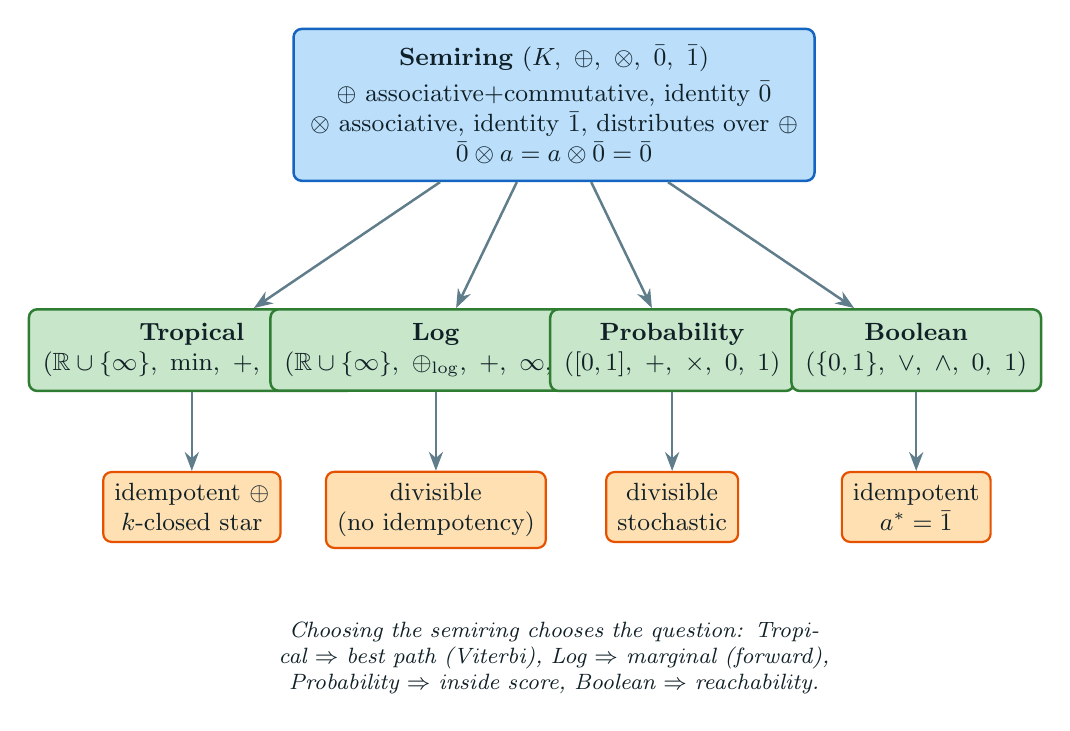
\begin{tikzpicture}[
    every node/.style={font=\small, text=ink},
    sig/.style={draw=foundationB, fill=foundation, rounded corners=3pt, align=center,
                inner sep=6pt, line width=0.9pt},
    sr/.style={draw=algorithmsB, fill=algorithms, rounded corners=3pt, align=center,
               inner sep=5pt, line width=0.9pt, minimum width=30mm},
    prop/.style={draw=speechB, fill=speech, rounded corners=3pt, align=center,
                 inner sep=4pt, line width=0.8pt},
    rel/.style={-{Stealth[length=2.4mm]}, draw=edge, line width=0.9pt},
  ]

  % the signature, at the top
  \node[sig] (sig) {\textbf{Semiring} $(K,\ \oplus,\ \otimes,\ \bar 0,\ \bar 1)$\\[2pt]
        $\oplus$ associative+commutative, identity $\bar 0$\\
        $\otimes$ associative, identity $\bar 1$, distributes over $\oplus$\\
        $\bar 0 \otimes a = a \otimes \bar 0 = \bar 0$};

  % the five core concrete semirings
  \node[sr, below=16mm of sig, xshift=-46mm] (trop)
        {\textbf{Tropical}\\ $(\mathbb{R}\cup\{\infty\},\ \min,\ +,\ \infty,\ 0)$};
  \node[sr, below=16mm of sig, xshift=-15mm] (log)
        {\textbf{Log}\\ $(\mathbb{R}\cup\{\infty\},\ \oplus_{\log},\ +,\ \infty,\ 0)$};
  \node[sr, below=16mm of sig, xshift=15mm]  (prob)
        {\textbf{Probability}\\ $([0,1],\ +,\ \times,\ 0,\ 1)$};
  \node[sr, below=16mm of sig, xshift=46mm]  (bool)
        {\textbf{Boolean}\\ $(\{0,1\},\ \vee,\ \wedge,\ 0,\ 1)$};

  \draw[rel] (sig) -- (trop);
  \draw[rel] (sig) -- (log);
  \draw[rel] (sig) -- (prob);
  \draw[rel] (sig) -- (bool);

  % property tags
  \node[prop, below=10mm of trop] (tropp) {idempotent $\oplus$\\ $k$-closed star};
  \node[prop, below=10mm of log]  (logp)  {divisible\\ (no idempotency)};
  \node[prop, below=10mm of prob] (probp) {divisible\\ stochastic};
  \node[prop, below=10mm of bool] (boolp) {idempotent\\ $a^{*}=\bar 1$};

  \draw[rel] (trop) -- (tropp);
  \draw[rel] (log)  -- (logp);
  \draw[rel] (prob) -- (probp);
  \draw[rel] (bool) -- (boolp);

  % caption
  \node[below=8mm of logp, xshift=15mm, text width=92mm, align=center, font=\footnotesize\itshape]
        {Choosing the semiring chooses the question: Tropical $\Rightarrow$ best path (Viterbi),
         Log $\Rightarrow$ marginal (forward), Probability $\Rightarrow$ inside score,
         Boolean $\Rightarrow$ reachability.};
\end{tikzpicture}
\end{document}
